\documentclass[12pt,oneside,a4paper]{article}
\usepackage{graphicx}
\usepackage{hyperref}
\begin{document}
% title (fold)
\begin{center}
{\LARGE \bfseries
 DIGIEZ --- Repair a corrupted video \\[0.3cm]
}
{\large
  \textsc{CentraleSupélec} --- Max Spahn --- P2018\\[0.7cm]
}
\end{center}
% title (end)

\section{Idea}
\label{sec:Idea}
Given the task of reconstructing the video, my first step was to frame the video in images so that i can treat them
individually. The main idea of my program is to compare individual pixel of all picture created that way. It is up 
to the user how many pixels he wants to be compared. An increase in pixel-number increases the accurancy of the 
program but causes a longer execution time. Once the images are put in the right order,you need to rebuild
the video.
\section{Technical details and problems}
\label{sec:Technical details and problems}
The programming language I am the most familiar with is C++, but I couldn't find a good library for 
my purpose. That's was the reason to choose \textsc{ffmpeg} as an external programe that needed to be combined with the cpp 
code in a bash file. On the other hand, the bash-file gave me much opportunities to automate the program. For example, 
it is kind difficult to compute the number of images created by ffmpeg, but a simple line in the bash-file counts the 
number of imagese. The number is than used for the iteration in the C++ program. 
The images are stored in the folder "images/" and they are named \textit{outxxx.bmp} where xxx is a place holder for the number
of a particular image. I decided to use the bitmap-format because it is one of the easiest to work with. The drawback is that 
there is now compression so the storage might become problematic if the video becomes too long.
Then the C++ program is executed with two command-line arguments, the first is the number of pixel
in each picture direction, the second is the number of images previously counted.
\begin{figure}
\begin{center}
	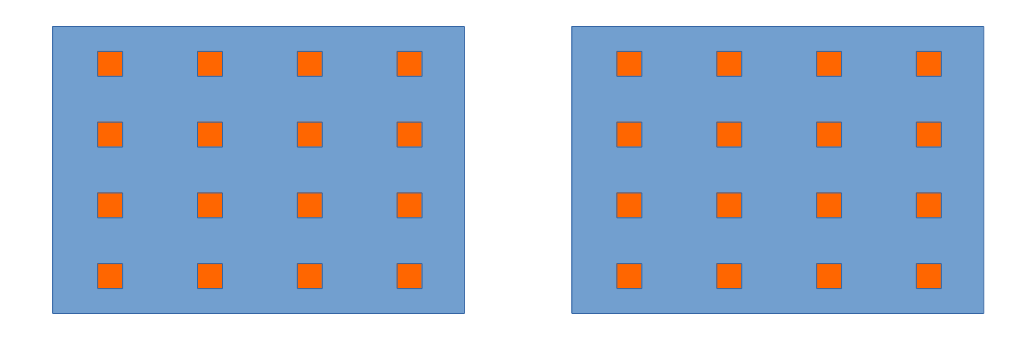
\includegraphics[scale=0.3]{explication_image.png}
\end{center}
\caption{Explanation of how two images are compared, for divison-factor div=4}
\label{fig:image}
\end{figure}

An array of changings is created to keep track of the order of the images. When every picture is put into the right position,
the image-files are renamed with regard to the changings-array. They are now called \textit{newxxx.bmp}.
\textsc{ffmpeg} is used a second time to reform the video, now in order.

\section{Problems}
\label{sec:Problems}
The major problem might be the compability with other operating systems than linux which i used for the program. On top of
that you need to preinstall \textsc{ffmpeg} and the C++-library for treating bitmaps. I put all the files needed to use 
\textsc{EasyBMP} in my github, \url{https://github.com/maxspahn/digiez}  with the other file, and \textsc{ffmpeg} can be downloaded on the link:
\url{https://ffmpeg.org/}. 
In case of problems I would be happy to talk to about my solution.



\end{document}
